\documentclass[11pt]{article}
\usepackage[a4paper,margin=1 in]{geometry}
\usepackage{graphicx}
\usepackage{caption}
\usepackage{subcaption}
\usepackage{listings}
\begin{document}

\title{Calculator using RaspberryPi \& LCD}
\author{R Rohith Reddy}
\date{\today}
\maketitle


\section{Objective}
	To make a simple calculator using Raspberry Pi where input is given through keyboard and display the whole operation on a 16x2 LCD display.
\section{Components Required}
\begin{enumerate}
 	\item Resistor-220Ohm
 	\item Raspberry Pi
 	\item 16x2 LCD display
 	\item Jumper wires
\end{enumerate}

\section{Introduction}
	\subsection{Raspberry Pi}
		The Raspberry Pi is a low cost, credit-card sized computer that plugs into a computer monitor or TV, and uses a standard keyboard, mouse, power supply and a micro SD card with installed Linux Distribution. It is a capable little device that enables people of all ages to explore computing, and to learn how to program in languages like Scratch and Python.
	\begin{figure}[h]
	\centering
		\begin{minipage}[t]{.5\linewidth}
		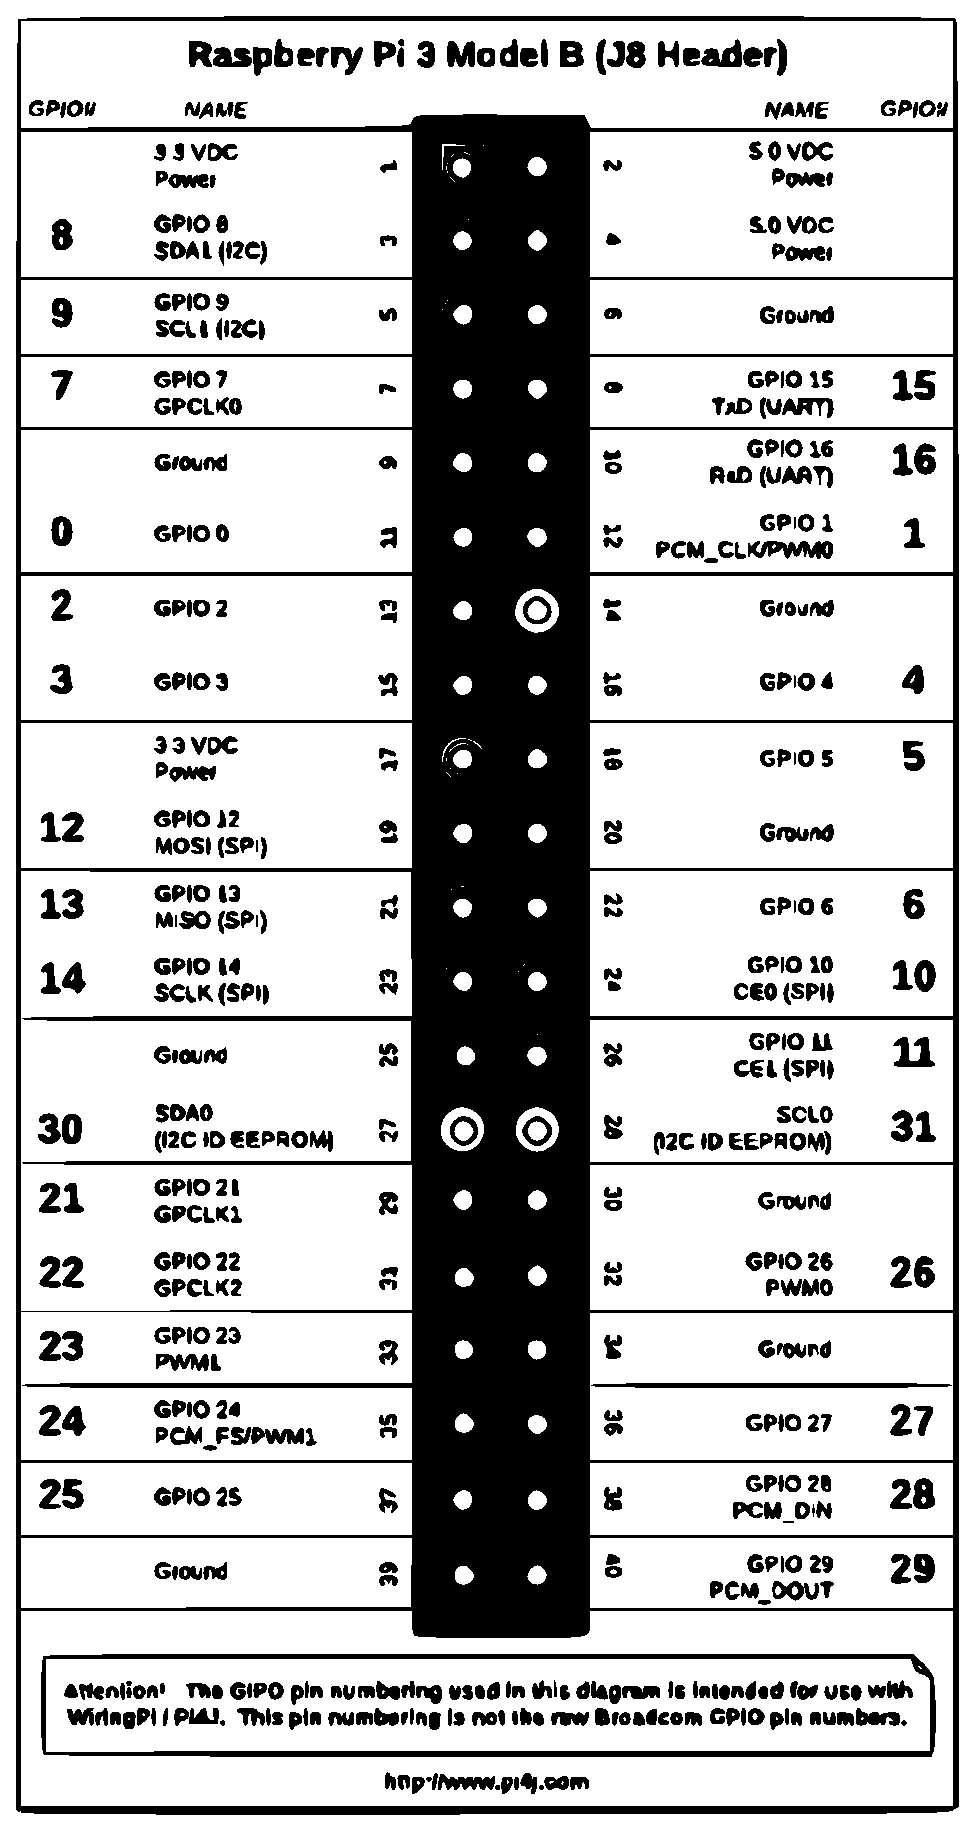
\includegraphics[scale=1]{rasp}
		\caption{ RPi 3B pin diagram}
		\label{fig:1}  
		\end{minipage}
	\end{figure}
	\subsection{16x2 LCD}
		LCD (Liquid Crystal Display) screen is an electronic display module and find a wide range of applications.A 16x2 LCD means it can display 16 characters per line and there are 2 such lines. In this LCD each character is displayed in 5x7 pixel matrix.
		
\section{Hardware Setup}
		
	\subsection{LCD to Raspberry Pi connections}
		\begin{enumerate}
		\item Connect the 5V pin i.e., pin 2 of the Raspberrry Pi to an extreme pin of the Breadboard. Let this pin be Vcc.
		\item Connect the GND pin i.e., pin 6 of the Pi to the opposite extreme pin of the Breadboard.

		
		\item Plug the LCD in Figure 1 to the bread-board.
		\item  Connect the 220$\Omega$ resistance from Vcc to pin 15 (Led+) of the LCD.
		\item Connect the raspberry pi pins to the LCD display as shown in the table below.
		\end{enumerate}


	\begin{table}[ht]
		\begin{minipage}[b]{0.56\linewidth}
			\centering
			\begin{tabular}{ |c|c| }
			\hline
			LCD pins & Raspberry Pi pins\\
			\hline
			GND & Ground\\
			Vcc & 5V\\
			Vss & Ground\\
			RS  & GPIO 25\\
			R/W & Ground\\
			EN  & GPIO 24\\
			DB4 & GPIO 23\\
			DB5 & GPIO 22\\
			DB6 & GPIO 21\\
			DB7 & GPIO 14\\
			LED+ & 5V\\
			LED- & Ground\\
			\hline
			\end{tabular}
			\caption{Raspberry Pi to LCD connections}
			\label{Table}			
	\end{minipage}	
	\hfill
		\begin{minipage}[h]{.5\linewidth}
		\centering
		\vspace{-5cm}
		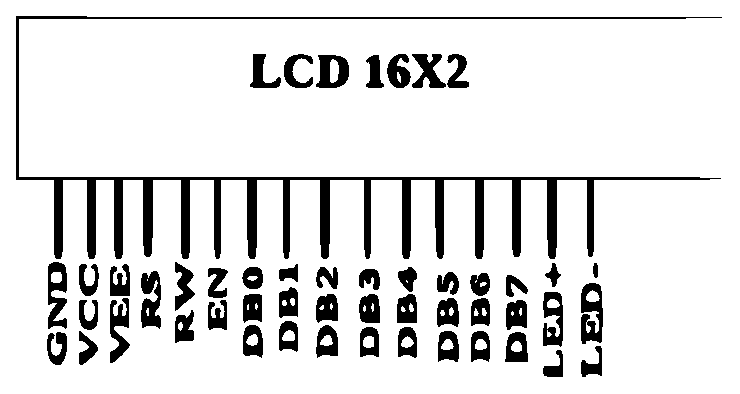
\includegraphics[scale=1]{lcd}
		\captionof{figure}{ LCD pin out}
		\label{fig:1}
	\end{minipage}
\end{table}
\section{Programming of Raspberry Pi}
	The code is written in C language by importing the wiring Pi library.\\
	WiringPi is a PIN based GPIO access library written in C for the BCM2835, BCM2836 and BCM2837 SoC devices used in all Raspberry Pi.\\
	Using the libraries lcd.h and wiringPi.h we can write the code for Pi.The code for the calculator is attached in the appendix H.
	

\section{Specifications of Calculator}
\begin{enumerate}

	\item Any number of inputs can be given to the calculator with any operations between the operands.
	\item The input can be a decimal number also and  can be a n digit number.
	\item If more than two inputs is given,it performs calculation of first two operands and the obtained result is used for next calculation with third operand and so on.\\
	For example if 2+3*4 is given it first adds 2+3=5 and this 5 is multiplied to 4 and the final result will be shown as 20.
	\item The result of the given input calculation along with the calculation entered is displayed on the LCD display for 4s.After 4s we can enter new calculation.
			
\end{enumerate}

\section{Conclusions}
A simple calculator with basic operations is made using a Raspberry Pi.GPIO pins of the Pi are used in making the hardware interface with the LCD.\\
Using C programming and wiring Pi,we can write code for the calculator by importing certain libraries.
		
\renewcommand\thesection{\Alph{section}}
\section{Appendix}
The C code for calculator:
\begin{lstlisting}
#include <stdio.h>
#include <wiringPi.h>
#include <lcd.h>

#define LCD_RS  25               //Register select pin
#define LCD_E   24               //Enable Pin
#define LCD_D4  23               //Data pin 4
#define LCD_D5  22               //Data pin 5
#define LCD_D6  21               //Data pin 6
#define LCD_D7  14               //Data pin 7
int main(){
	int i,count,op[100],j=0,k,sign[100],l,m=0,n=0;
	float h[100],res;
	char arr[100],num[100][100];		
	int lcd;               
    wiringPiSetup();        
    lcd = lcdInit (2, 16, 4, LCD_RS, LCD_E, LCD_D4, LCD_D5, LCD_D6, LCD_D7, 0, 0, 0, 0);
    while()
    {
    lcdPosition(lcd, 5, 0); 
    lcdPuts(lcd, "Simple");
	lcdPosition(lcd, 3, 1);
	lcdPuts(lcd, "Calculator");
	printf("Enter the Calculation\n");
	for(i=0;i<100;i++)
	{
		scanf("%c",&arr[i]);
		if(arr[i]=='=')
		{
			count=i;
		    break;
		}
	}
	lcdClear(lcd);
	for(i=0;i<count;i++)
	{
		lcdPosition(lcd, i, 0); 
		if(arr[i]=='+'||arr[i]=='-'||arr[i]=='*'||arr[i]=='/'||arr[i]=='=')
		{
			lcdPrint(lcd, "%c",arr[i]);
		}
		else
		{
			lcdPrint(lcd,"%c",arr[i]);
		}
	}
    
    for(i=0;i<count+1;i++)
	{
		if(arr[i]=='+'||arr[i]=='-'||arr[i]=='*'||arr[i]=='/'||arr[i]=='=')
		{
			op[j]=i;
			sign[j]=arr[i];
			j=j+1;
		}
	}	
	for(n=0;n<j;n++)
	{	
		if(n==0)
		{
			for(k=0;k<op[n];k++)
			{
				num[n][k]=arr[k];
			}
		}
		else 
		{
			for(k=0;k<op[n]-op[n-1]-1;k++)
			{
				num[n][k]=arr[op[n-1]+1+k];
			}
		}
		
	}
	
	for(i=0;i<j;i++)
	{
		if(i==0)
		{
			sscanf(num[i], "%g", &h[i]);
		}
		else 
		{
			sscanf(num[i], "%g", &h[i]);
		}	
	}
	k=0;
	for(i=0;i<j-1;i++)
	{
		switch(sign[k])
		{
		case '+':
			res=h[i]+h[i+1];
			break;
		case '-':
			res=h[i]-h[i+1];
			break;
		case '*':
			res=h[i]*h[i+1];
			break;
		case '/':
			res=h[i]/h[i+1];
			break;
		}
		h[i+1]=res;
		k=k+1;
	}
	printf("result=%g\n",res);
	lcdPosition(lcd, 0, 1); 
    lcdPrint(lcd, "Result:%0.6g",result);
    sleep(4);
	lcdClear(lcd);
	
		
	}
	return 0;
}

\end{lstlisting}
\end{document}